\clearpage
\chapter{\textbf{Beispiele}}\label{beispiele}
\addtocontents{toc}{\vspace{0.8cm}}

\section{Formale Struktur der Arbeit}

Formal gliedert sich jede Arbeit in  
\begin{itemize}
\item Vorspann
\item Hauptteil
\item Nachspann 
\item Anhang
\end{itemize}
\vspace{0.5cm}

Als Vorspann werden alle Seiten bezeichnet, die vor der Einleitung liegen. Der Vorspann 
besteht aus den Seiten 

\begin{itemize}
\item Titelseite (Einband), 
\item Leerseite,
\item Erklärung über die eigenständige Anfertigung und ggf. Geheimhaltungserklärung, 
\item evtl. Danksagung, 
\item Kurzfassung der Arbeit,  
\item  Inhaltsverzeichnis.
\end{itemize}
\vspace{0.5cm}

Informationen zur Darstellung und Lösung der gestellten Aufgabe gehören in den Hauptteil. Zusätzliches Material, das den Textfluss unterbricht, gehört in den Anhang.  Der Nachspann besteht aus 

\begin{itemize}
\item Quellenverzeichnis, 
\item Abkürzungsverzeichnis, 
\item Bild- und Tabellenverzeichnis.  Der Anhang enthält zusätzliches Informationsmaterial, das für das Verständnis der Arbeit 
\end{itemize}

das für das Verständnis der Arbeit nicht wesentlich ist, jedoch eine Vertiefung ermöglicht. Zusätzliches Tabellenmaterial, Ergebnisse von Parametervariationen, Programm-Code, Messreihen etc., also alles, was den Textfluss unterbricht, wird hier platziert. Der Anhang kann dazu gegliedert werden in A1, A2 etc.\\  

\textbf{Erklärung}\\
In der Erklärung über die selbständige Anfertigung sind Monat Jahr durch die aktuellen Werte zu ersetzen. (Vollständige, handschriftliche Unterschrift) ist zu löschen. Jedes Exemplar ist zu unterschreiben. \\

\textbf{Danksagung}\\ 
Bei der Anfertigung ihrer Arbeit werden Studierende i. d. R. von Betreuern in Betrieben und von einem betreuenden Professor begleitet. Vielfach sind sie auf die Unterstützung von Werkstätten angewiesen. In der Danksagung kann der Studierende sich für diese Unterstützung bedanken.  \\

\textbf{Kurzfassung}\\ 
Die Kurzfassung gibt auf ein bis zwei Seiten die wesentlichen Inhalte und Ergebnisse der Abschlussarbeit wieder. Sie gliedert sich inhaltlich in 
\begin{itemize}
\item das behandelte Gebiet, 
\item das Ziel der Arbeit, 
\item die Untersuchungsmethode,  
\item die Ergebnisse und 
\item die Schlussfolgerungen.
\end{itemize}

Die Kurzfassung enthält keine Schlussfolgerungen oder Bewertungen, die über die Inhalte der Kapitel der Arbeit hinausgehen. Alle Aussagen der Kurzfassung finden sich in ausführlicher Form in der Arbeit wieder. Die Kurzfassung erhält keine Kapitelnummer. \\

\textbf{Titelseite}\\
Die Titelseite steht als download-Datei auf der Internetseite des Prüfungssekretariats zur 
Verfügung. Die grau hinterlegten Felder sind zu ergänzen oder zu modifizieren. Wird kein 
Firmenlogo gedruckt, erscheinen Datum und ggf. übrige Zeilen zentriert.\\

\textbf{Inhaltsverzeichnis}\\
Das Inhaltsverzeichnis führt alle Kapitelnummern, Überschriften und zugehörige Seitenzahlen des Hauptteils, Nachspanns und Anhangs auf. Es erleichtert das Auffinden von Abschnitten und gibt eine Übersicht über die Gliederung der Arbeit. Das Inhaltsverzeichnis trägt die Überschrift \glq Inhalt\grq{}. Alle Kapitelnummern stehen links bündig. Einrückungen sind nicht vorgesehen. Die Überschriften und ggf. Folgezeilen beginnen an einer einheitlichen Fluchtlinie. Seitenzahlen enden rechtsbündig an einer einheitlichen Fluchtlinie. [DIN 1421] Nur die Kapitel von Einleitung bis Bewertung erhalten Kapitelnummern. Die Überschriften aller übrigen Abschnitte werden an der linken Fluchtlinie der Kapitelnummern ausgerichtet. \\

\textbf{Quellenverzeichnis}\\
Das Quellenverzeichnis listet alle verwendeten Quellen der Arbeit auf. Anhand des Quellenverzeichnisses muss eine Beschaffung der Literatur möglich sein. Internetquellen sind vollständig zu bezeichnen und mit Datum zu versehen. \\

\textbf{Abkürzungsverzeichnis}\\
Das Abkürzungsverzeichnis enthält alle verwendeten Abkürzungen, die nicht dem allgemeinen Sprachgebrauch angehören. PC, Lkw, z. B. etc. werden nicht aufgeführt. Ebenso werden die verwendeten Formelzeichen mit ihrer Bedeutung aufgeführt. Werden Abkürzungen nur in dem Kapitel verwendet, wo sie eingeführt und erklärt werden, kann das Abkürzungsverzeichnis entfallen, \ac{zb}. \\

\textbf{Bild- und Tabellenverzeichnis}\\
Ein Bild- und Tabellenverzeichnis sind nur erforderlich, wenn die Bilder und Tabellen unabhängig vom Text gefunden werden sollen. Ein Bildverzeichnis enthält Bildnummer, Bildunterschrift und Seitenzahl. 

\newpage

\section{Was ganz Allgemeines}
\subsection{Welche Dateien braucht man wirklich?}
Ein Compilerlauf erzeugt eine Unmenge Dateien. Die meisten integrierten Tex-Umgebungen bieten einen Befehl zum Aufräumen, der alles löscht, was nicht zu Ihrem Projekt gehört.

Folgende Dateien dürfen nie gelöscht werden

\begin{tabu}{|X[0.5] | X[3] |}
\hline
\rowfont{\bfseries} Endung & Inhalt \\
\hline
tex & Ihre Tex-Quelldateien\\
bib & Ihre Literaturdatenbank(en)\\
\hline
\end{tabu}
und natürlich alles an Material (Bilder etc.), was Sie einbinden. Fast alle anderen Dateien dürfen (und sollten gelegentlich) entsorgt werden, insbesondere

\begin{tabu}{|X[0.5] | X[3] |}
\hline
\rowfont{\bfseries} Endung & Inhalt \\
\hline
aux & Hilfsdateien\\
toc & Erzeugte Verzeichnisse\\
lot & \\
lof & \\
out & \\
blg & Log-Datei des Bibtex-Laufs \\
log & Log-Datei des pdflatex-Laufs\\
\hline
\end{tabu}


\subsection{Was ist eigentlich Blindtext?}

\blindtext
\subsection{Wie macht man Aufzählungen?}
Zum Beispiel als
\begin{itemize}
\item einfache
\item unnummerierte
\item Liste
\end{itemize}

oder auch als numerierte Liste mit
\begin{enumerate}
\item Erstens
\item Zweitens 
\item Drittens
\end{enumerate}

Möchten Sie nun mehrere Aufzählungen verschachteln, müssen Sie einfach innerhalb der ersten itemize-Umgebung eine weitere Umgebung initiieren. Das Ganze stellt sich für vier Ebenen dann wie folgt dar:

\begin{itemize}
\item 1. Ebene
\begin{itemize}
\item 2. Ebene
\begin{itemize}
\item 3. Ebene
\begin{itemize}
\item 4. Ebene
\end{itemize}
\end{itemize}
\end{itemize}
\end{itemize}


\section{Tabelle}
\subsection{Ein Buch mit sieben Siegeln}

Es gibt eine unüberschaubare Menge an Styles für Tabellen. Den einfachsten Einstieg erhalten Sie, wenn Sie nicht die tabular-Umgebung, sondern die tabu-Umgebung verwenden. Hier ein Beispiel, Tabelle \ref{tabelle1}.

\begin{table}
\caption{Tabellen beschriftet man \underline{oberhalb}}
\label{tabelle1}
\tabulinesep=3pt  % ein bisschen Platz schaffen
\begin{tabu} to 0.8\textwidth {| X[0.5c] | X[2r] | X[3l]|}
\hline
\rowfont{\bfseries} Nr & Aktion & Formel\\ 
\hline
1 & Bachelorarbeit schreiben &
$G(s) = \frac{1}{(s-s_p)^n}$
\\\hline
2 & Heiraten &
$G(s) = \frac{s\omega_0^2}{s^2+2D\omega_0 s + \omega_0^2}$ 
\\\hline
3 & Baum pflanzen &
$F(s) = \mathscr L \{f (t)\} = \int\limits_0^{\infty} f (t) \, e^{-s t} \text{d}t$
\\
\hline
\end{tabu}
\end{table}



\subsection{Verdammt nochmal, ich will selbst entscheiden}

... wohin meine Tabelle oder mein Bild kommt.

table und figure sind so genannte Float-Umgebungen, d.~h. Latex entscheidet, wo sie hinkommen und geht davon aus, dass es Ihnen egal ist, weil Sie die Objekte mit \textbackslash caption beschriften und über \textbackslash label und \textbackslash ref dorthin verweisen.

Wenn Sie das mögen (und damit sind Sie nicht alleine), verwenden Sie stattdessen andere Umgebungen, wie z.B. par oder center. Um dennoch eine Bild- bzw. Tabellennummer zu erhalten, benutzen Sie statt \textbackslash caption den Befehl \textbackslash captionof. Sie Beispiel Tabelle \ref{tabelle2} \underline{direkt nach diesem Absatz}.

\begin{table}[H]
\begin{center}
\captionof{table}{Tabellen beschriftet man \underline{oberhalb}}
\label{tabelle2}
\begin{tabu} to 0.8\textwidth {| X[0.5c] | X[2r] | X[3l]|}
\hline
\rowfont{\bfseries} Nr & Aktion & Formel\\ 
\hline
1 & Bachelorarbeit schreiben &
$G(s) = \frac{1}{(s-s_p)^n}$
\\\hline
2 & Heiraten &
$G(s) = \frac{s\omega_0^2}{s^2+2D\omega_0 s + \omega_0^2}$ 
\\\hline
3 & Baum pflanzen &
$F(s) = \L \{f (t)\} = \int\limits_0^{\infty} f (t) \, e^{-s t} \text{d}t$
\\
\hline
\end{tabu}
\end{center}
\end{table}

\textbf{Tabellen}\\
In Tabellen werden gleichartige Größen $f_k(x_i)$ in einer Spalte stellenwertrichtig untereinander angeordnet. Im Spaltenkopf steht die Bezeichnung der jeweiligen Größe $f_k$. Wird nur ein Formelzeichen im Spaltenkopf aufgeführt, ist neben oder unter der Tabelle eine Legende erforderlich. Die Vorspalte enthält die Bezugsgröße $ x_i$. Spaltenköpfe und Vorspalte werden durch Linien von den Tabellenfeldern getrennt. Die Spalten und Zeilen können  durch weitere Linien getrennt werden. Jede Tabelle erhält eine Tabellenüberschrift, die das Wort „Tabelle“ gefolgt von einer Nummer und der Bezeichnung der Tabelle enthält. Aus der Bezeichnung muss der Inhalt der Tabelle deutlich werden. 


%% Tabelle mit Fußnote
%% Verschiedene Symbole
\newcommand{\cmark}{\ding{51}}%
\newcommand{\xmark}{\ding{55}}%

\newcounter{mytabfnValuee}
\setcounter{mytabfnValuee}{\value{footnote}}
\begin{table}[H]
\caption{ Tabellenüberschrift mit Referenzierung \cite{web}}
\label{Systemparametergnss}
\centering
\begin{tabularx}{\textwidth}{|r|X|X|X|X|}
\hline
\textbf{text} & \textbf{text} & \textbf{text} & \textbf{text} & \textbf{text}\\
\hline
Bachelorarbeit schreiben \footnotemark & 1 & 2 & 3 & 4\\
\hline
Heiraten & \xmark & \xmark & \cmark & \cmark \\
\hline
\end{tabularx}
\end{table}
  \stepcounter{mytabfnValuee}%
    \footnotetext[\value{mytabfnValuee}]{%
       fast geschafft}%

%% neue Tabelle mit multicolumns

\begin{table}[h]
\caption{Zusammenfassung der Messdaten}
\label{tab:zed_imu}
\begin{tabularx}{\textwidth}{|l|*{6}{X|}}
\hline
\textbf{} & \multicolumn{3}{c|}{\textbf{Beschleunigung}} & \multicolumn{3}{c|}{\textbf{Winkelgeschwindigkeit}} \\
\cline{2-7}
\textbf{ } & \textbf{x in m/s²} & \textbf{y in m/s²} & \textbf{z in m/s²} & \textbf{x in 1/s} & \textbf{y in 1/s} & \textbf{z in 1/s} \\
\hline
\textbf{count} & 75000 & 75000 & 75000 & 75000 & 75000 & 75000 \\
\hline
\textbf{mean} & 0,095 & 0,165 & 9,789 & -0,000 & 0,000 & 0,000 \\
\hline
\textbf{std} & 0,009 & 0,009 & 0,009 & 0,001 & 0,001 & 0,001 \\
\hline
\textbf{min} & 0,055 & 0,126 & 9,753 & -0,006 & -0,006 & -0,006 \\
\hline
\textbf{max} & 0,137 & 0,219 & 9,824 & 0,006 & 0,006 & 0,006 \\
\hline
\end{tabularx}
\end{table}
\vspace{0.2cm} % Abstand unter dem Tab

\newpage
\subsection{Formeln}

Kurze Formeln können im laufenden Text angegeben werden, wenn der Zeilenabstand nicht beeinflusst wird, z. B. aus der Drehzahl n folgt die Winkelgeschwindigkeit $\omega = 2 \cdot \pi \cdot n$.\\

Alle übrigen Formeln werden in eine eigene Zeile gedruckt. Sie werden nicht zentriert, sondern eingerückt und rechts mit einer Formelnummer versehen.

\begin{align}
((\Delta T_i +\Delta t) \cdot v)^2  = (X_i -X_E)^2+(Y_i -Y_E))^2+(Z_i -Z_E))^2 \  ; i=1,2,3,4 
\end{align}\\

\hspace*{12mm}$\Delta T_i$ \hspace{2,2cm} gemessene Laufzeiten \\
\hspace*{12mm}$\Delta t$ \hspace{2,4cm} unbekannte Messabweichung\\
\hspace*{12mm}$v$ \hspace{2,6cm} Ausbreitungsgeschwindigkeit\\
\hspace*{12mm}$X_i,Y_i,Z_i$ \hspace{1,3cm} bekannten Koordinaten\\
\hspace*{12mm}$X_E,Y_E,Z_E$ \hspace{1cm} unbekannte Koordinaten\\

\vspace{1.0cm}


Griechische Buchstaben können in Latex folgendermaßen erzeugt werden. \\

$\alpha$ $\beta$ $\gamma$ $\delta$ $\epsilon$ $\zeta$ $\eta$ $\theta$ $\iota$ $\kappa$ $\lambda$ $\mu$ $\nu$ $\xi$ $\pi$ $\rho$ $\sigma$ $\tau$ $\upsilon$ $\phi$ $\chi$ $\psi$ $\omega$ \\

\newpage


 %% Beispiel für das Einfügen einer Abbildung
\subsection{Einfügen von Bildern}

Der richtige Tex-perte tex't auch seine Bilder, z. B. so wie in Bild \ref{bild2}

% Define block styles
	\tikzstyle{Baustein} = [rectangle, draw, 
    text width=3.5cm, text centered, rounded corners, minimum height=1cm]
	\tikzstyle{Baustein2} = [rectangle, draw, 
    text width=7cm, text centered, rounded corners, minimum height=1cm]
	\tikzstyle{Baustein3} = [rectangle, draw, 
    text width=9cm, text centered, rounded corners, minimum height=1cm]
	\tikzstyle{Baustein4} = [rectangle, draw, 
    text width=3.5cm, text centered, rounded corners, minimum height=4cm]
	 
	\tikzstyle{line} = [draw, -latex']
	\tikzstyle{line2} = [draw]

\begin{figure}[H]
\begin{center}
\begin{tikzpicture}[node distance = 1.5cm, auto]
    % Place nodes
 	   \node [Baustein] (M) {Name};
 	   \node [Baustein, below of=M] (W) {Name};
 	   \node [Baustein, below of=W] (F) {Name};
  	  \node [Baustein, below of=F] (P) {Name};
  	  \node [Baustein2, below of=P] (S) {Name};
  	\coordinate (D) at (-4,-6);

    % Draw edges

   	 \path [line](S)--(P);
	\path [line](P) -- (F);
	\path [line](F) -- (W);
	\path [line](W)-- (M);
	\path[line2] (M)-|(D);
  	 \path[line] (D)--(S); 
\end{tikzpicture}
\caption{figure}{Ein mit tikz gezeichnetes Flussdiagramm}
\label{bild2}
\end{center}
\end{figure}

\blindtext

\subsection{Ganze Bilder}
text text text text text text text text text text text text text text text text text text text text text text text text text text text text text text text text text text text text text text text text text text text text text text text text text text text text text text text text text text text text text text text text text text text text text text text text

\begin{figure}[H]
	\centering
		\includegraphics[width=1.0\textwidth]{pic/fhac_2.jpg}
	\caption{Bildunterschrift}
	\label{fig:fhaachen}
\end{figure}
\vspace{1cm} % Abstand unter dem Bild

\newpage


\subsection*{Textumflossene Bilder }


text text text text text text text text text text text text text text text text text text text text text text text text text text text text text text text text text text text text text text text text text text text text text text text text text text text text text text text text text text text text text text text text text text text text text text text text.\\
Hier ein Zitat \cite{book}. \\
Zwei Zitate \cite{book}, \cite{manual}.\\

\begin{wrapfigure}{l}{8cm}
  \includegraphics[width=8cm]{pic/fhac_2.jpg}
  \caption{Bildunterschrift mit Referenzierung nach \cite{article}}
  \label{fig:bild}
\end{wrapfigure}

Bild Referenzierung \ref{fig:bild}.  text text text text text text text text text text text text text text text text text text text text text text text text text text text text text text text text text text text text text text text text text text text text text text text text text text text text text text text text text text text text text text text text text text text text text text text text text text text text text text text text text text text text text text text text text text text text text text text text text text text text text text text text text text text text text text text text text text text text text text text text text text text text text text text text text text text text text text text text text text text text text text text text text text text text text text text text text text text text text text text text text text text text text text text text text text text text text text text text text text text text text text text text text text text text text text text text text text text text text text text text text text text text text text text text text text text text.

\newpage

\subsection{Graphen und Bilder mit TikZ}


TikZ ist ein Package, mit dem sich Grafiken erstellen lassen. Dabei wird je Kommando eine Linie oder ein Shape generiert.  Auf der Internetseite von Overleaf \cite{tikz} wird das Package recht gut erklärt.

\begin{figure}[h!]
	\centering
	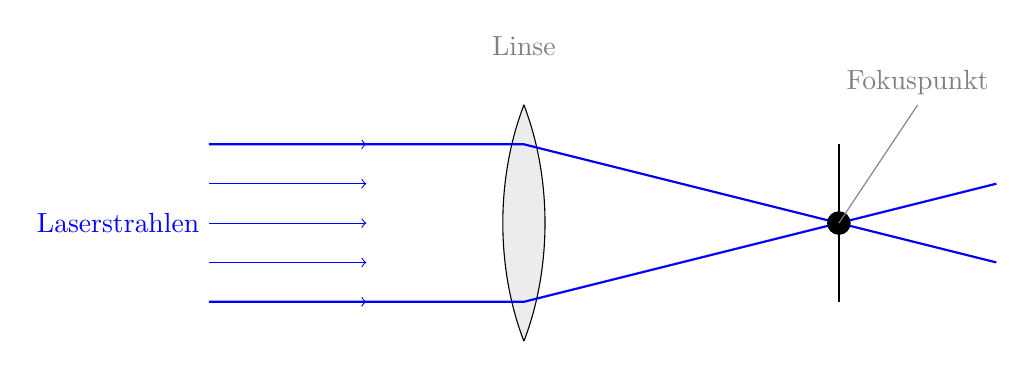
\begin{tikzpicture}
		\draw[line join=round,fill=gray!15] (4,-4.5) arc (-30:30:2 and 3) arc (150:210:2 and 3);  % Linse]
		\node [above, gray] at (4, -1) {Linse}; % Text Linse über der Linse
		\draw [thick, blue] (0,-2) -- (4, -2) -- (10, -3.5); 
		\draw[thick, blue] (0, -4) -- (4, -4) -- (10, -2.5);
		\draw[thick, black] (8, -2) -- (8, -4);
		\fill[black] (8,-3) circle (0.15);
		\draw [gray] (8, -3) -- (9, -1.5) node [above] {Fokuspunkt};
		\draw[blue, ->] (0, -3) node [left]{Laserstrahlen} -- (2, -3);
		\draw[blue, ->] (0, -2) -- (2, -2);
		\draw[blue, ->] (0, -4) -- (2, -4);
		\draw[blue, ->] (0, -2.5) -- (2, -2.5);
		\draw[blue, ->] (0, -3.5) -- (2, -3.5);
		
		
	\end{tikzpicture}
	\caption{Fokuspunkt eines Lasers, erstellt mit TikZ}
	\label{graph:laser_fokus}
\end{figure}


\newpage

\section{Verwendung von Literatur}

Um das korrekte Zitieren kümmert sich bibtex. Legen Sie eine Datei (Datenbank) mit Ihrer Literatur als Datei \verb+[name].bib+ an. Darin nehmen Sie für jede Referenz eine Quellenangabe auf.

Tipp: Die meisten Literaturdatenbanken bieten die Möglichkeit, bibtex-Datensätze zu exportieren.

Wenn Sie auf Quellen, wie z.B. diese Webreferenz \cite{web} oder auch dieses Buch \cite{book} verweisen, erscheinen die entsprechenden Titel perfekt formatiert im Literaturverzeichnis.

Damit alle Referenzen stimmen, muss man ggf. pdflatex und bibtex mehrfach aufrufen. Sicher ist die folgende Reihenfolge
\begin{enumerate}
\item pdflatex. Erzeugt die *.aux-Datei, die bibtex benötigt
\item bibtex. Erzeugt Dateien, die pdflatex einbindet
\item pdflatex
\item pdflatex (Ggf. auf Fehlermeldungen schauen. Nach dem zweiten Lauf sollte alles okay sein)
\end{enumerate}
